%!TEX root = ../thesis.tex

% \vspace{-20pt}

\section{本章の概要}
% 本章では,\ref{sec:nav-sys}節でシステムの概要を示す.また,\ref{sec:real-robot}節で実ロボットにおける歩行者の位置計算の詳細,\ref{sec:nav-usage}節でナビゲーションにおける予測結果の利用方法について述べる.

本章では,ナビゲーションシステムの概要,実ロボットにおける歩行者の位置計算の詳細,およびナビゲーションにおける予測結果の利用方法について述べる.まず,\ref{sec:nav-sys}節でシステムの概要を示し,次に\ref{sec:real-robot}節で実ロボットにおける歩行者の位置計算の詳細を説明する.最後に,\ref{sec:nav-usage}節でナビゲーションにおける予測結果の利用方法について述べる.

% \newpage

\section{システム概要}\label{sec:nav-sys}
\figref{Fig:nav-system}に,本研究で構築したナビゲーションシステムの概要図を示す.本システムは以下に示す3つの主要モジュールで構成される.

\begin{itemize}
  \item \textbf{制御モジュール} \\
  制御モジュールは,ROS Navigation stackの主要コンポーネントであるmove\_baseにより構成される.
  センサデータと目標位置を受け取り,適切な制御指令をロボットに送信する.
  \item \textbf{認識モジュール} \\
  認識モジュールは,YOLOを用いて歩行者の検出・追跡し,観測時間分のデータをまとめて時系列データとして出力する.
  \item \textbf{予測モジュール} \\
  予測モジュールは,認識モジュールから受け取ったデータをもとに,\ref{chap:proposed_method}章で述べたネットワークを用いて歩行者の位置を予測する.その後,制御モジュールのglobal\_costmapの独自レイヤで予測結果をコストマップに反映させる.
\end{itemize}

% \newpage

% \vspace*{15pt}

\vspace{-10pt}

\begin{figure}[H]
  \centering
 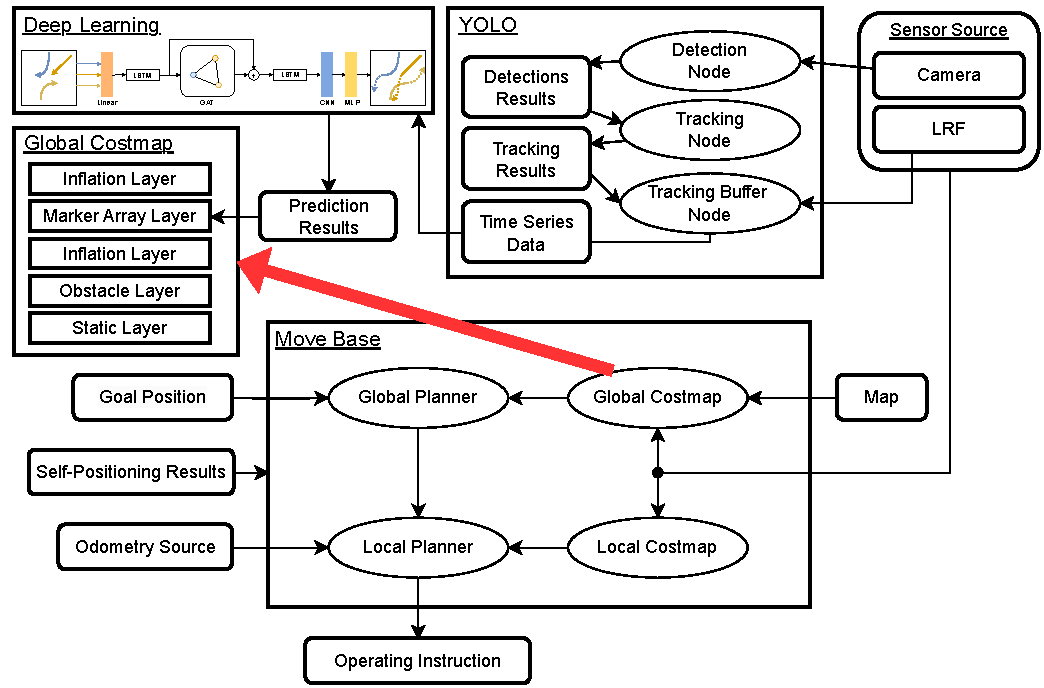
\includegraphics[keepaspectratio, scale=0.77]
      {images/application_system.pdf}
 \caption{Navigation system overview}
 \label{Fig:nav-system}
\end{figure}

\vspace{-30pt}

\section{実ロボットにおける歩行者の位置計算}\label{sec:real-robot}
\figref{Fig:ped2pos}に,俯瞰視点のデータセットと実ロボット上での歩行者位置推定のイメージを示す.ここで,データセットとはETH\cite{pellegrini2009you-eth}やUCY\cite{lerner2007crowds-ucy}データセットのように,俯瞰視点のデータセットのことを指す.\figref{Fig:ped2pos-dataset}のように,データセットは俯瞰視点の映像と各時刻における歩行者のワールド座標系上の位置が含まれている.しかし,実ロボットで歩行者位置を推定する際は,ロボットがセンサを通じて取得した情報のみを用いてワールド座標系の位置を算出しなければならない.\figref{Fig:ped2pos-realrobot}の例のように,1人称視点で撮影した画像中の歩行者の位置を座標変換することで,ワールド座標系上の位置を得る.これにより,データセットと同じ形式の歩行者の位置データが得られ,データセットで学習したモデルを再学習することなく実ロボット上に適用できる.

\begin{figure}[H]
  \centering
  \begin{minipage}{0.85\textwidth}
    \centering
    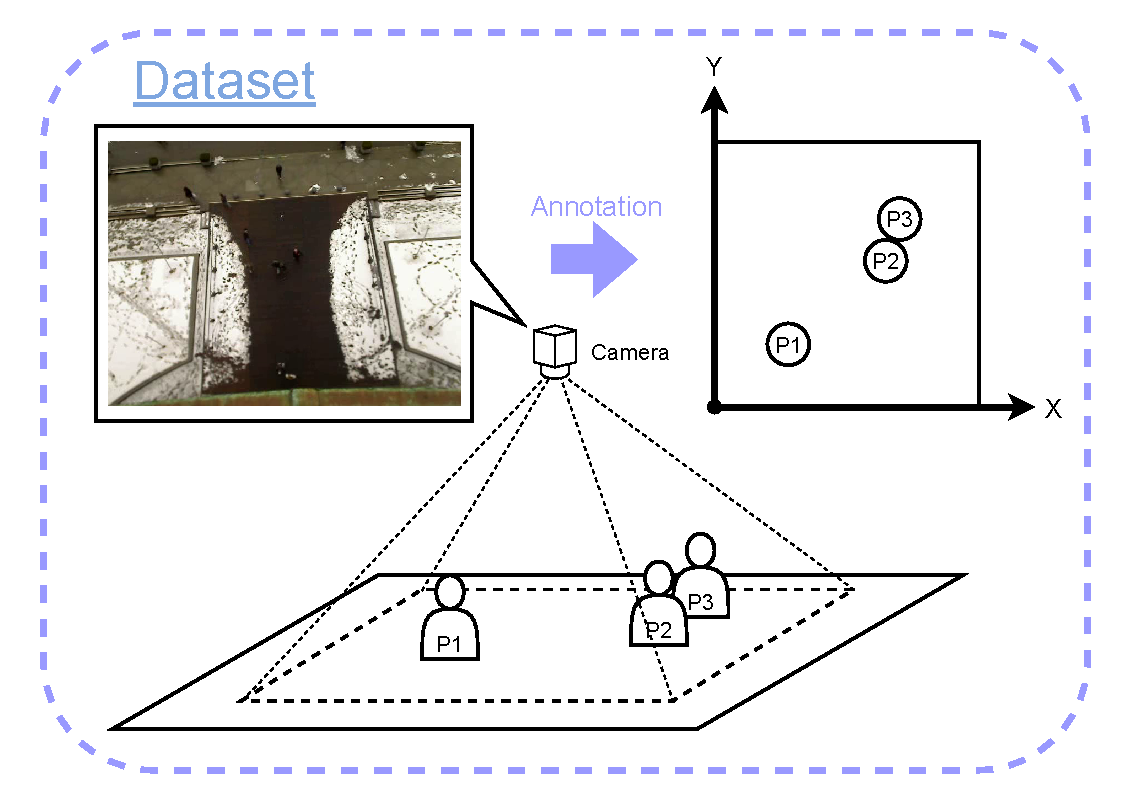
\includegraphics[width=\linewidth]{images/ped2pos-dataset.pdf}
    \subcaption{Pedestrian position calculation on dataset}
    \label{Fig:ped2pos-dataset}
  \end{minipage}
  \hfill
  \begin{minipage}{0.85\textwidth}
    \centering
    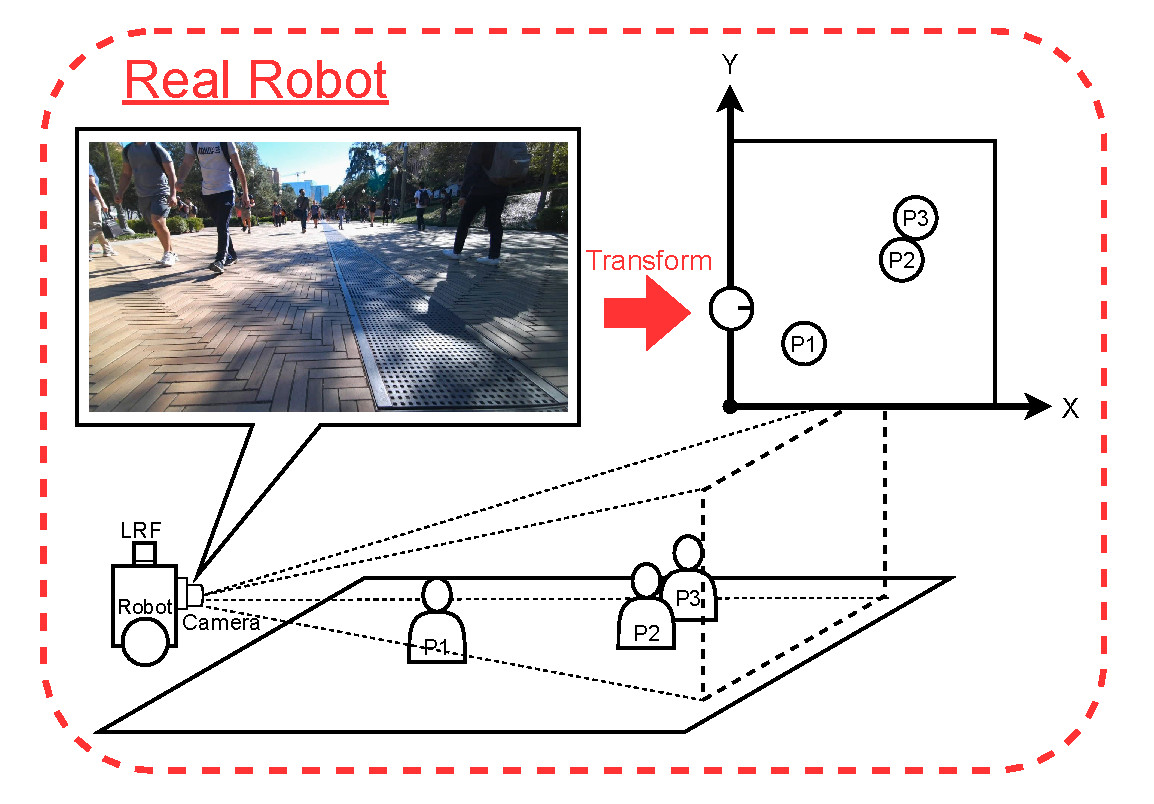
\includegraphics[width=\linewidth]{images/ped2pos-realrobot.pdf}
    \subcaption{Pedestrian position calculation on real robot}
    \label{Fig:ped2pos-realrobot}
  \end{minipage}
  \caption{Pedestrian position calculation: (a) on dataset, (b) on real robot}
  \label{Fig:ped2pos}
\end{figure}
% \protect\footnotetext[8]{\cite{pellegrini2009you-eth}より画像を引用}
% \protect\footnotetext[9]{\cite{karnan2022socially-scand}より画像を引用}

\newpage

本研究での実ロボットにおける歩行者の位置計算の流れと詳細を以下に示す.

\begin{enumerate}
  \item \textbf{RGBカメラ画像とLRFデータを取得} \\
  ロボット前方に取り付けたRGBカメラから歩行者の画像を取得し,同時にLRF(Laser Range Finder)から周囲の距離データを得る.いずれも歩行者の位置推定に必要となる情報を提供する.

  \item \textbf{YOLOで人間検出} \\
  YOLO\cite{redmon2016you-yolo}は,高速・高精度な物体検出アルゴリズムであり,RGBカメラ画像から歩行者を検出する.本研究では,YOLOv9\cite{wang2025yolov9}の学習済みモデル(yolov9c.pt)を使用し,画像上で歩行者の位置を特定する.

  \item \textbf{検出した個体の画像上での角度を計算} \\
  検出した歩行者の画像上での位置をもとに,式\eqref{yolo-ang}に従いロボットカメラの視野内における角度$\theta_{camera}$を求める.
  \begin{equation}
    \theta_{camera} = - \cfrac{(x_{center} - \cfrac{w_{img}}{2}) \cdot fov_{horizontal}}{W_{img}} \label{yolo-ang}
  \end{equation}

  ここで,$w_{img}$は画像の幅,$fov_{horizontal}$はカメラの水平視野角,$x_{center}$が検出バウンディングボックスの中心の$x$座標である.計算後,$\theta_{camera}$を$-\pi \text{から} \pi$の範囲に正規化する.

  \item \textbf{計算した角度とLRFデータからロボットとの相対位置を計算} \\
  画像上で得られた角度情報に対応するLRFデータの要素を取り出す.そして,そのデータを用いて歩行者とロボットとの相対位置を計算する.LRFはロボットからの距離情報を提供し,歩行者の正確な位置を特定するために使用される.

  \item \textbf{相対位置をワールド座標へ座標変換} \\
  最後に,得られた相対位置をワールド座標系に変換する.この座標変換は,ロボットのナビゲーションシステムのmapフレームに基づいて行われる.ワールド座標系での位置が特定されることで,ロボットは歩行者の位置を正確に把握し,適切なナビゲーションを行うことができる.
\end{enumerate}

\section{ナビゲーションにおける予測結果の利用方法}\label{sec:nav-usage}
\figref{Fig:global-costmap}に示すように,グローバルコストマップに独自のレイヤとしてMarker Array Layerを追加した.このレイヤでは,0.4秒ごとに受け取る予測結果をコストマップへ反映する.
\ref{sec:decoder}節で述べたとおり,予測結果のデータ形式はガウス分布を構成する5次元の要素である.本研究では,そのガウス分布からサンプリングした軌道を予測結果としてコストマップに反映する.
\figref{Fig:costmap-flow}のように,各レイヤでの処理を積み重ねて,最終的なグローバルコストマップを生成する.グローバルコストマップを拡張したのは,\ref{sec:navigation-stack}項で述べたように,多くのロボットで使用されているNavigation stackで予測結果を容易に利用できるようにするためである.

\begin{figure}[H]
  \centering
 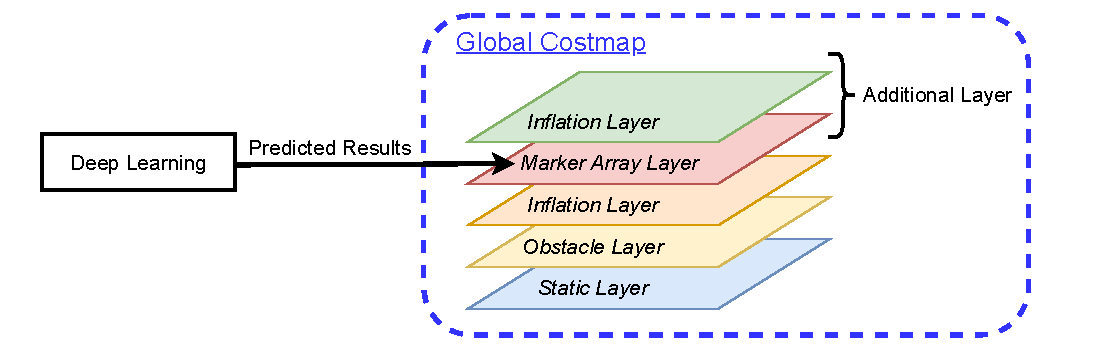
\includegraphics[keepaspectratio, scale=0.65]
      {images/layer.pdf}
\caption{Global costmap with costom layer}
 \label{Fig:global-costmap}
\end{figure} 

\vspace{-20pt}

\begin{figure}[H]
  \centering
 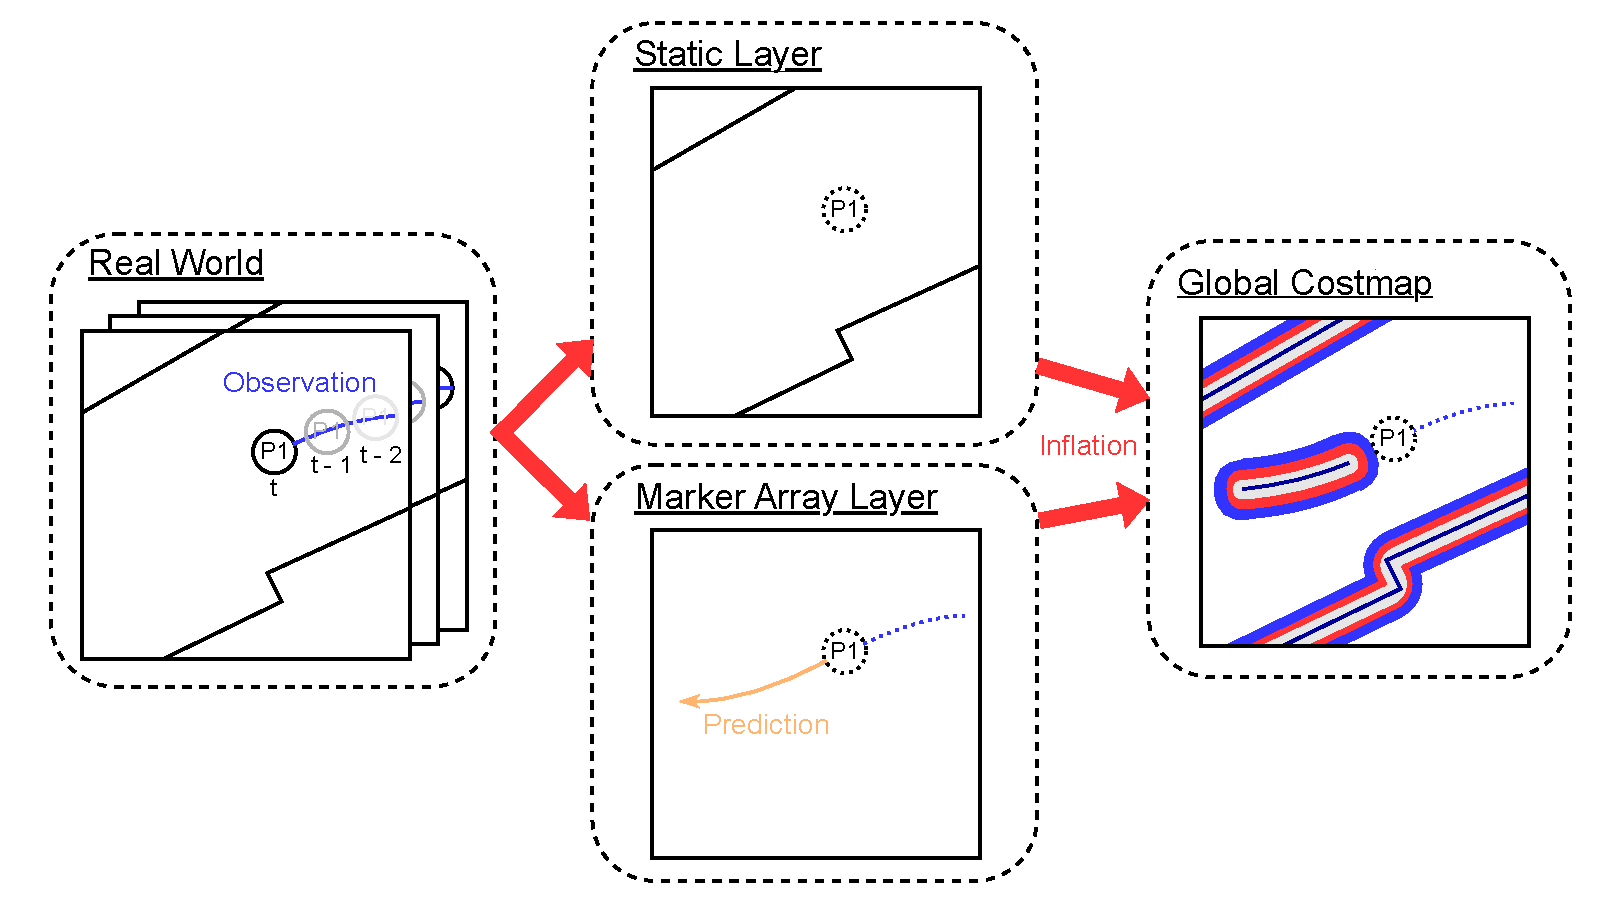
\includegraphics[keepaspectratio, scale=0.45]
      {images/costmap-image.pdf}
\caption{Process each layer to generate a global costmap}
 \label{Fig:costmap-flow}
\end{figure} 


\newpage
